% File:    report.tex
% Brief:   report for CS 354 Project 2
% Author:  G. Mcgaffin (23565608@sun.ac.za)
% Author:  J. P. Visser (21553416@sun.ac.za)
% Date:    2022-08-11

\documentclass[10pt, a4paper]{article}

\usepackage{booktabs}
\usepackage{graphicx}
\graphicspath{ {./images/exp1/}{./images/exp2/}{./images/exp3/} }

\title{CS 354 Project 2: Reliable Blast User Datagram Protocol (RBUDP)}
\author{Group 41: \vspace{0.5em} \\
        G. Mcgaffin (23565608@sun.ac.za) \vspace{0.3em} \\
        J.\ P.\ Visser (21553416@sun.ac.za)}
\date{\vspace{1em} 19 August 2022}

\begin{document}

\maketitle
\newpage

\tableofcontents
\newpage

% --- Introduction ----------------------------------------------------------- %

\section{Introduction}
\label{sec:intro}

We were tasked with developing two programs for transferring files via TCP and
RBUDP. The one program must act as the sender and the other as the receiver.

\subsection{Sender Requirements}
\label{subsec:sender-req}

The sender had the following implementation requirements:
\begin{enumerate}
  \item Must have a simple GUI.
  \item Must be able to select a file to transfer.
  \item Files must be transferred to the receiver across the local network using
    RBUDP.
  \item Files must be transferred to the receiver across the local network using
    TCP.
  \item RBUDP must make use of datagram packets for data transfer and may use a
    TCP connection for signalling only.
  \item RBUDP datagram packets must contain unique sequence numbers.
\end{enumerate}

\subsection{Receiver Requirements}
\label{subsec:receiver-req}

And the receiver had the following implementation requirements:
\begin{enumerate}
  \item Must have a simple GUI.
  \item Must be able to receive files from the sender.
  \item Must show the progress of incoming files.
  \item Must be able to handle dropped packets and out of order RBUDP datagram
    packets appropriately.
\end{enumerate}

\subsection{Overview}
\label{subsec:overview}

In this document we will provide a complete view of our implementation, by
discussing its design (\S\ref{sec:design}), giving a breakdown of the files into
which it is organized (\S\ref{sec:file-desc}), and providing a high level
description, with more details where appropriate, of the flow of execution of
the two programs which it comprises (\S\ref{sec:prog-desc}).

By our own evaluation, we are confident that our implementation meets all the
requirements, which makes it unnecessary to include a section dedicated to
unimplemented features. We will, however, discuss features we have implemented
additional to the requirements in \S\ref{sec:add-feat}.

Furthermore, we will also cover issues we encountered during the development
process (\S\ref{sec:issues}), experiments we have conducted (\S\ref{sec:exp}),
compilation and execution of the two programs (\S\ref{sec:comp-exec}), as well
as the libraries we made use of (\S\ref{sec:libs}).

% --- Additional Features ---------------------------------------------------- %

\section{Additional Features}
\label{sec:add-feat}

\subsection{Sender Cannot Connect to Receiver}
\label{subsec:send-cant-connect}

If for whatever reason the sender cannot establish a connection with the
receiver when the user presses the send button, then an alert is shown to inform
the user of this issue.\footnote{We also included various other alerts (in both
the sender and receiver) to provide the user with feedback as they interact with
the system.}


\subsection{Transfer Success Status}
\label{subsec:trans-suc-stat}

In our implementation, once the sender starts sending a file to the receiver,
the transfer cannot be stopped via the GUI. However, the user can still
terminate the program by closing the window or by sending a kill signal to it
via the command-line. Terminating the program will cause the receiver to lose
its connection to the sender, and it will consider the transfer complete, even
though that cannot be the case.

In the earlier versions of our implementation we simply showed the user an alert
to notify them that the transfer had been \emph{completed} (i.e., the sender was
sending something, but it is not anymore), without indicating whether the
transfer was \emph{successful}. 

So in order to provide a better experience to the user running the receiver, we
added an extra check that, once a file tranfer has ended (either by completing,
or by the sender being terminated), compares the number of bytes written to the
byte size of the file that was transferred. Using this check we can inform the
user not only about the completion of the transfer, but also whether it was
successful.

% --- File Descriptions ------------------------------------------------------ %

\section{File Descriptions}
\label{sec:file-desc}

\subsection{Sender Files}
\label{subsec:sender-file-desc}

\subsubsection{\texttt{Sender.java}}
\label{subsubsec:send.java}

This file implements the sender's networking logic. It contains a static
function for sending files to the receiver, either via TCP or RBUDP. It also
contains a private helper function for writing \texttt{short int} values to a
specified position in a \texttt{byte} array.

\subsubsection{\texttt{SenderGUI.java}}
\label{subsubsec:send-gui.java}

Implements the sender's graphical user interface, and calls the \texttt{send}
function defined in \texttt{Sender.java} to send files to the receiver.

\subsection{Receiver Files}
\label{subsec:receiver-file-desc}

\subsubsection{\texttt{Receiver.java}}
\label{subsubsec:recv.java}

Contains one static function for receiving files (via TCP or RBUDP), another for
returning the transfer progress as a \texttt{double} value between 0 and 1
(inclusive), and one for reading a \texttt{short int} value from a specified
position in a \texttt{byte array}.

\subsubsection{\texttt{ReceiverGUI.java}}
\label{subsubsec:recv-gui.java}

This file implements the graphical user interface for the receiver. It
repeatedly calls the \texttt{receive} and \texttt{getProgress} functions defined
in \texttt{Receiver.java} to receive files and report on the progress of the
transfer operation.

% --- Program Description ---------------------------------------------------- %

\section{Program Description}
\label{sec:prog-desc}

\subsection{Sender}
\label{subsec:prog-desc-sender}

\begin{enumerate}
  \item When \texttt{SenderGUI} is run, it processes the command-line arguments
    passed to it, and sets up the graphical user interface.
  \item Key elements of the user interface include a button the user can press
    to select a file, using the system file chooser; a menu for selecting which
    protocol to use; and the send button, which the user can press to initiate
    the file transfer when they are happy with the file that they have chosen.
  \item Upon pressing the send button, certain UI elements are disabled (like
    the browse button, for instance). The file tranfer is then initiated on a
    new thread, so that the UI can remain responsive.
  \item The file transfer is started by invoking the \texttt{send} function,
    defined in the \texttt{Sender.java} file, passing to it the name of the file
    to send, destination host address, destination port, the protocol to use
    (TCP or RBUDP), blast size, and the packet size.
  \item The sender function will then attempt to connect to the receiver. If
    successful it will communicate the same information from step 4 to the
    receiver via TCP.
  \item If the file is being transferred via TCP, the file will be opened for
    reading, a number of bytes equal to the packet size will be read into a
    buffer, and sent to the receiver. This will continue until the end of the
    file is reached.
  \item If the file is sent via RBUDP, the process is a bit more complex:
    \begin{enumerate}
      \item The sender will first create a number of packets equal to the blast
        size.
      \item It creates each packet by writing a sequence number, and data
        length to the first four bytes (two for the sequence number and two for
        the data length) of a byte array. Then it read file data into the
        remaining number of elements in the array.\footnote{File data is read
        as needed, not all at once.}
      \item The send function then enters a \texttt{while} loop, where it waits
        for the receiver to provide a list of all the missing packets, then
        sends those packets to the receiver via UDP, and then goes back to
        waiting for the missing packets list. This goes on until all of the
        packets in the current ``blast" are completely tranferred.
      \item The process then restarts, and continues until the entire file is
        sent to the receiver.
    \end{enumerate}
  \item When the file tranfer is complete, the previously disabled UI elements
    are re-enabled and the user can again select a file to send.
  \item Various UI alerts are used throughout the program to give feedback to
    the user.
  \item The user can stop a file transfer before it is finished by terminating
    the application.
  \item Upon termination all resources are closed.
\end{enumerate}

\subsection{Receiver}
\label{subsec:prog-desc-receiver}

\begin{enumerate}
  \item When \texttt{ReceiverGUI} is run it processes its command-line arguments
    and sets up the graphical user interface for interacting with the receiver.
  \item Key elements of the UI include a buttton that can be pressed in order
    to select a directory for saving files to; and a button to start listening
    for incoming files. The selection of the directory is handled by the system
    file chooser.
  \item When the receive button is pressed, certain UI elements are disabled to
    prevent the user from accidently doing something wrong (e.g., pressing the
    receive button multiple times, thereby starting up multiple threads
    listening for incoming files). On a new thread, the \texttt{receive}
    function is called and it waits for a connection from the sender.
  \item Upon connecting with the sender, the receiver first receives some basic
    information about the transfer that is going to take place. (See point 4
    of \S\S\ref{subsec:prog-desc-sender}.)
  \item If the transfer takes place using TCP, then the receiver will simply
    read the byte data it receives from its socket input stream to disk until it
    reaches the end of the stream.
  \item If the file is being received via RBUDP, the following steps are
    followed:
    \begin{enumerate}
      \item The receiver starts the conversation by telling the sender that
        all of the packets are missing. It does this by sending, via TCP, a
        \texttt{boolean} array whose length is equal to the blast size with
        all of its elements set to \texttt{false}.
      \item The sender then sends all of the packets in the current ``blast".
      \item The receiver tries to receive all \texttt{DatagramPacket}s, and
        takes note of the number of packets, and which packets it successfully
        captures.
      \item It then revises the list of packets the sender needs to retransmit,
        and sends the updated list to the sender.
      \item This process goes on until all packets in the ``blast" are received.
        Then the data is extracted from the packets and written to the disk.
      \item The process then restarts, and continues until the entire file is
        received.
    \end{enumerate}
  \item While the \texttt{receive} function is busy receiving the file on one
    thread, the \texttt{getProgress} function (also from the \texttt{Receiver}
    class) is repeatedly called to determine the percentage of the file that
    have been written to storage in order to update a progress bar.
  \item Various UI alerts are used throughout the program to provide feedback to
    the user.
  \item The user can stop a file transfer before it is finished by terminating
    the program.
  \item Upon termination all resources are closed.
\end{enumerate}

% --- Experiments ------------------------------------------------------------ %

\section{Experiments}
\label{sec:exp}

\subsection{Comparison of TCP and RBUDP Throughput}
\label{subsec:comp-tcp-rbudp-throughput}

\subsubsection{Experiment}
\label{subsubsec:exp-1}

Determine which protocol, TCP or RBUDP, has higher throughput.

\subsubsection{Hypothesis}
\label{subsubsec:exp-1}

During the development process we found RBUDP to reliably be slower than TCP
when testing under similar conditions. Therefore, we expect the throughput of
TCP to be higher than that of RBUDP.

\subsubsection{Test}
\label{subsubsec:test-1}

For both the TCP and RBUDP protocols, capture a set number of packets using
the command-line utility \texttt{tcpdump}, and compare the average number of
bytes per second using Wireshark (see Figure \ref{fig:exp1-1} and Figure
\ref{fig:exp1-2}). The experiment is carried out on the local network in order
to prevent (or at least mitigate) packet dropping from influencing the results.

\begin{figure}
  \centering
  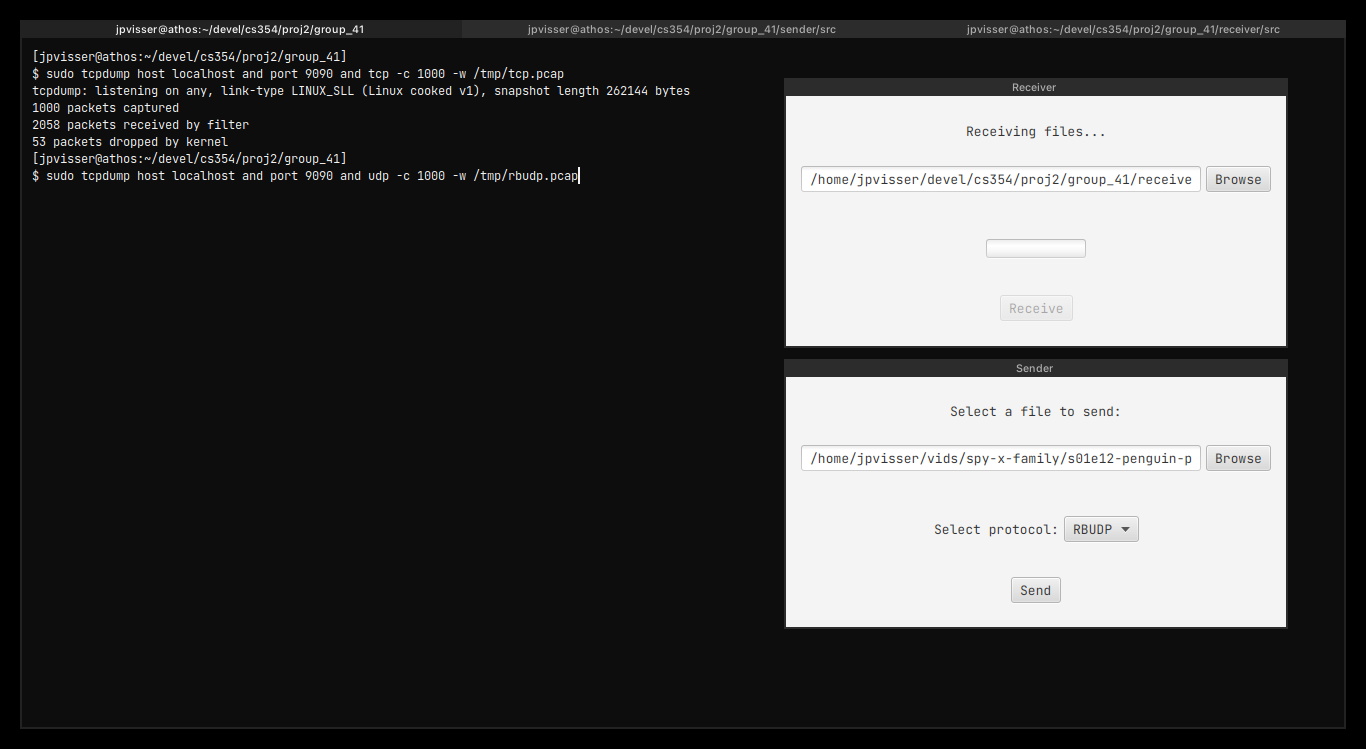
\includegraphics[width=12cm]{exp1-1}
  \caption{Transferal of a file using RBUDP while capturing 1000 packets using
  \texttt{tcpdump}. (Note that all images in this document have a very high
  resolution, so the reader may zoom in on them for closer inspection.)}
  \label{fig:exp1-1}
\end{figure}

\begin{figure}
  \centering
  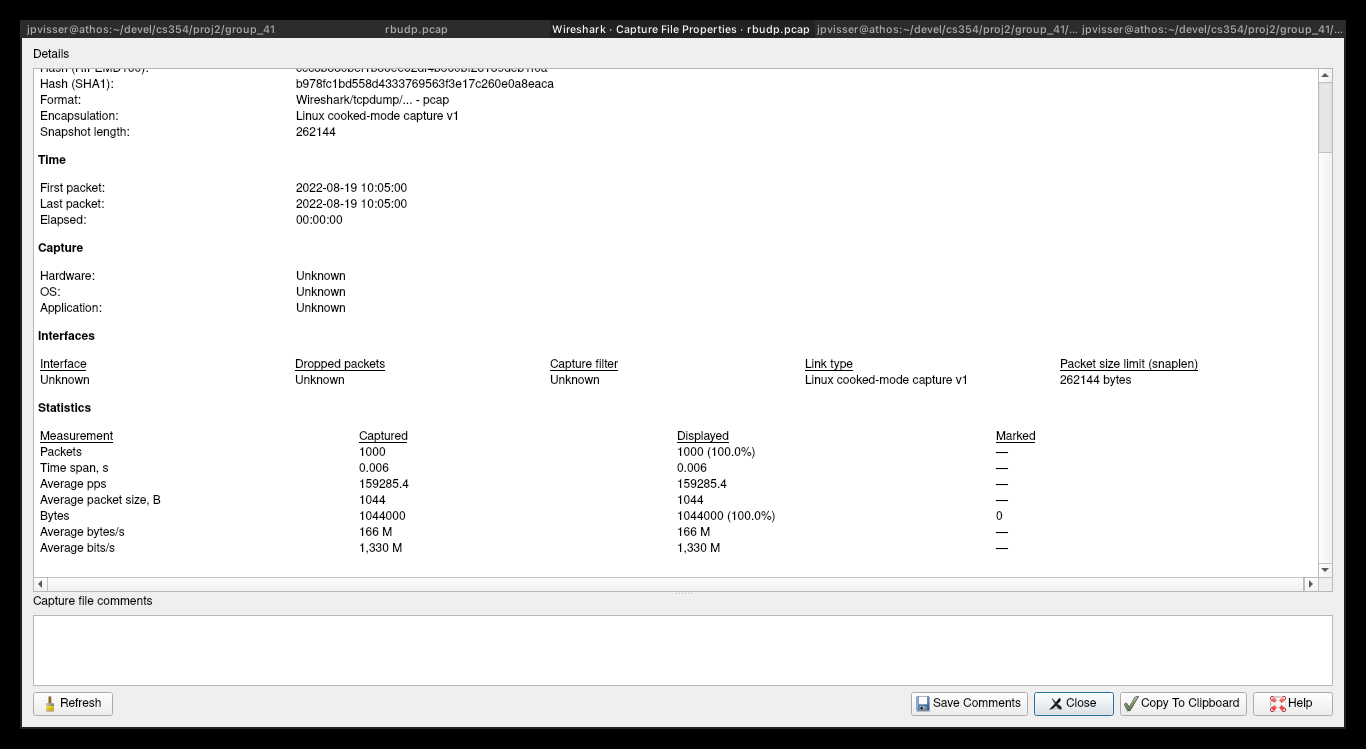
\includegraphics[width=12cm]{exp1-3}
  \caption{Wireshark's ``Capture File Properties" view of the 1000 packets
  captured using \texttt{tcpdump}}
  \label{fig:exp1-2}
\end{figure}

\subsubsection{Findings}
\label{subsubsec:findings-1}

Somewhat surprisingly, we found that the RBUDP protocol has higher throughput
than the TCP protocol. Wireshark's data analysis indicated that RBUDP has, on
average, a 30.7\% higher throughput (on the local network of the machine we used
to conduct the experiment).

This contradicts the faster transfer rate we see for TCP. From the data analysis
we saw that despite sending 1000 byte packets at a time, both for TCP and RBUDP,
TCP transferred packets with a size of 25676 bytes on average. Our suspicion is
that, at a lower level, the network architecture collects the bytes written to
the socket output stream and only sends them once a packet with a large enough
size to meet certain requirements (most likely for the sake of efficiency) can
be created.

\subsection{RBUDP Transfer Rate}
\label{subsec:rbudp-trans-rate}

\subsubsection{Experiment}
\label{subsubsec:exp-2}

Determine the correlation of blast size and transfer rate for RBUDP.

\subsubsection{Hypothesis}
\label{subsubsec:exp-2}

We expect the blast size and transfer rate to be positively correlated, but only
up to a certain point, whereafter the correlation will become negative. We also
expect this correlation to be influenced by the packet size. Our expectation is
based on the logic that a larger blast size will cause data to arrive more
rapidly for the receiver to process, which will result in a higher transfer
rate. However, once the blast size is increased beyond a certain threshold, a
large number of packets will be dropped while the receiver is busy processing a
packet, which will result in a greatly decreased transfer rate.

\subsubsection{Test}
\label{subsubsec:test-2}

Run the sender program with different blast sizes while keeping the packet size
constant. Measure the time it takes to complete a file transfer in each case
(using the same file in each case). Then compare the times. Conduct this
experiment on a local network to avoid introducing confounding factors.

We used the blast sizes listed in Table \ref{tab:blast-time}, and kept the
packet size fixed at 1000 bytes. To measure transfer times we used the
\texttt{stat} command-line utility, part of the \texttt{coreutils} package, to
get the received file's \texttt{Birth} and \texttt{Change} times. The transfer
time can be found by taking the difference between these two times. See Figure
\ref{fig:exp2-1} and Figure \ref{fig:exp2-2}.

\begin{figure}
  \centering
  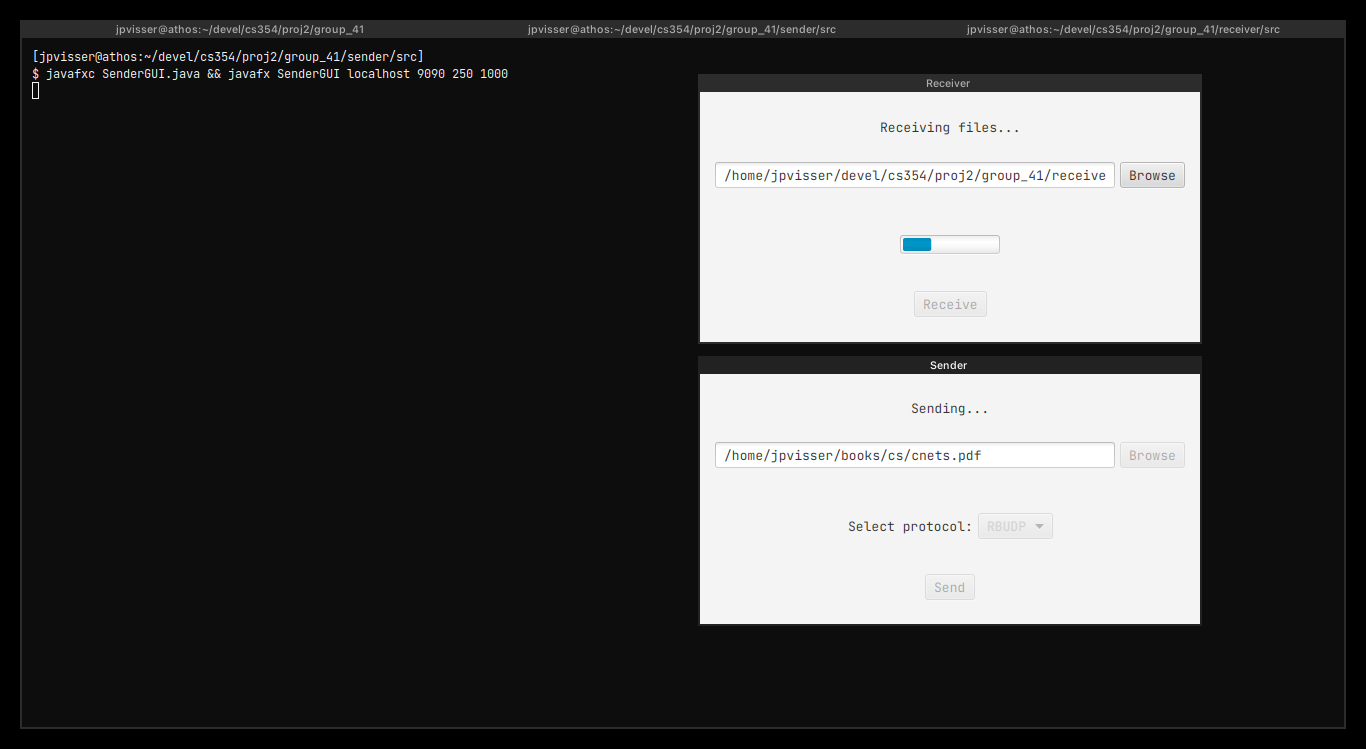
\includegraphics[width=12cm]{exp2-1}
  \caption{The sender using a blast size of 250 to transfer a file to the
  receiver.}
  \label{fig:exp2-1}
\end{figure}

\begin{figure}
  \centering
  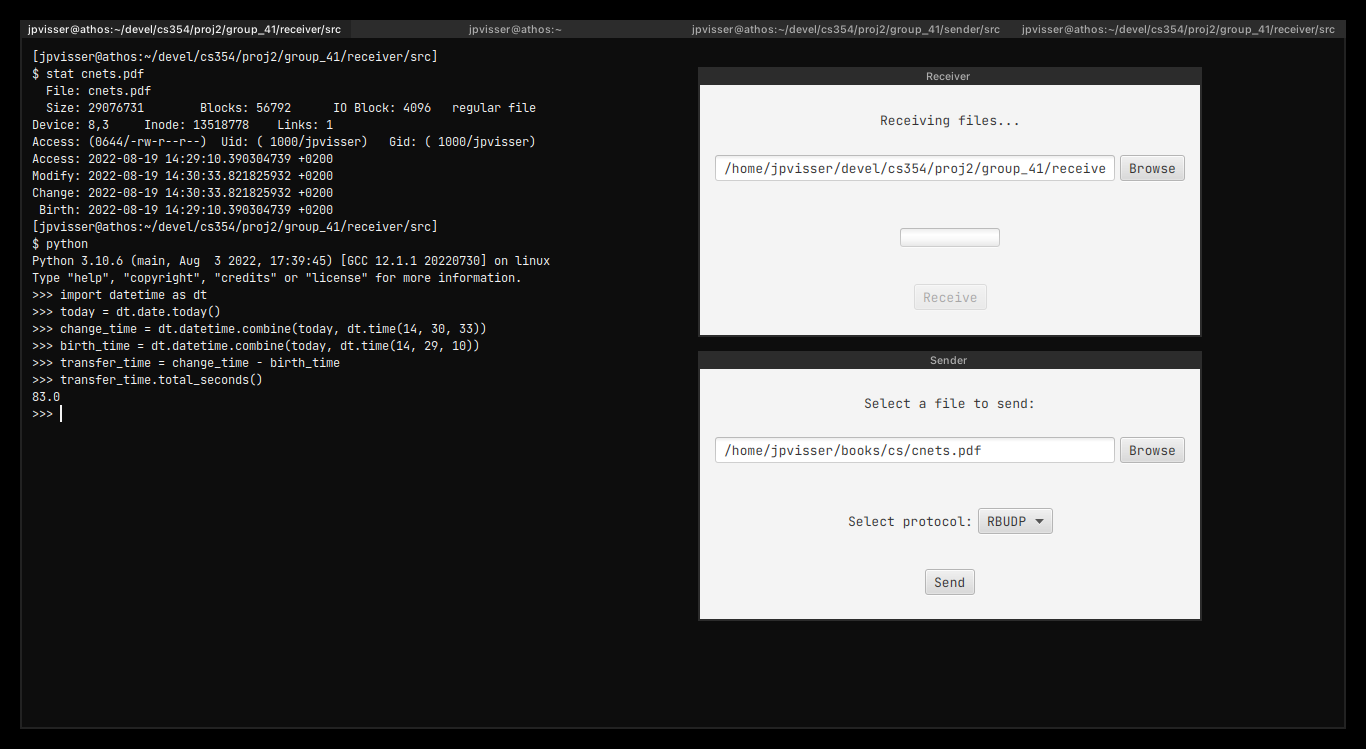
\includegraphics[width=12cm]{exp2-2}
  \caption{After the file transfer, using a blast size of 250, is successfully
  completed, the \texttt{stat} utility is used to determine the \texttt{Birth}
  and \texttt{Change} times. The number of seconds to complete the transfer is
  then calculated in the Python interpreter.}
  \label{fig:exp2-2}
\end{figure}

\subsubsection{Findings}
\label{subsubsec:findings-2}

Our hypothesis turned out to be correct. Table \ref{tab:blast-time} shows that
as the blast size increases exponentially, the transfer time decreases at a
similar rate, which indicates that blast size and transfer rate are positively
correlated. At a blast size of 128000, the transfer took too long for us to wait
until its completion. Therefore, there must be a tipping point, somewhere between
64000 and 128000, where the correlation becomes negative.

\begin{table}
  \centering
  \begin{tabular}{@{}rr@{}}
    \toprule
    Blast Size & Time (s) \\
    \midrule
    1000 & 70 \\
    2000 & 40 \\
    4000 & 20 \\
    8000 & 17 \\
    16000 & 10 \\
    32000 & 5 \\
    64000 & 7 \\
    128000 & $\infty$ \\
    \bottomrule
  \end{tabular}
  \caption{The different blast sizes and their associated transfer times in
  seconds when transferring a 29 MB file. The transfer time for blast size
  128000 is indicated as $\infty$, because the transfer took too long to
  complete -- in fact, it never even reached the point where the receiver could
  write data to the file.}
  \label{tab:blast-time}
\end{table}

\subsection{RBUDP Packet Size}
\label{subsec:rbudp-pkt-sz}

\subsubsection{Experiment}
\label{subsubsec:exp-3}

Determine the correlation between packet size and transfer rate for RBUDP.

\subsubsection{Hypothesis}
\label{subsubsec:exp-3}

We expect results similar to those seen in \S\S\ref{subsec:rbudp-trans-rate}. We
expect the transfer rate to increase as the packet size increases, and to then
again decrease beyond a certain threshold.

\subsubsection{Test}
\label{subsubsec:test-3}

Run the sender multiple times using a different packet size for each run, while
keeping the blast size constant. Measure the time it takes for each file
transfer to finish, and determine the correlation, if any. Be sure to use a
local network to ensure that packet dropping does not influence the results.

We conducted the experiment using a constant blast size of 1000 packets, and the
different packet sizes shown in Table \ref{tab:packet-time}. Figure
\ref{fig:exp3-1} shows the result obtained by running the sender with a packet
size of 10000.

\begin{figure}
  \centering
  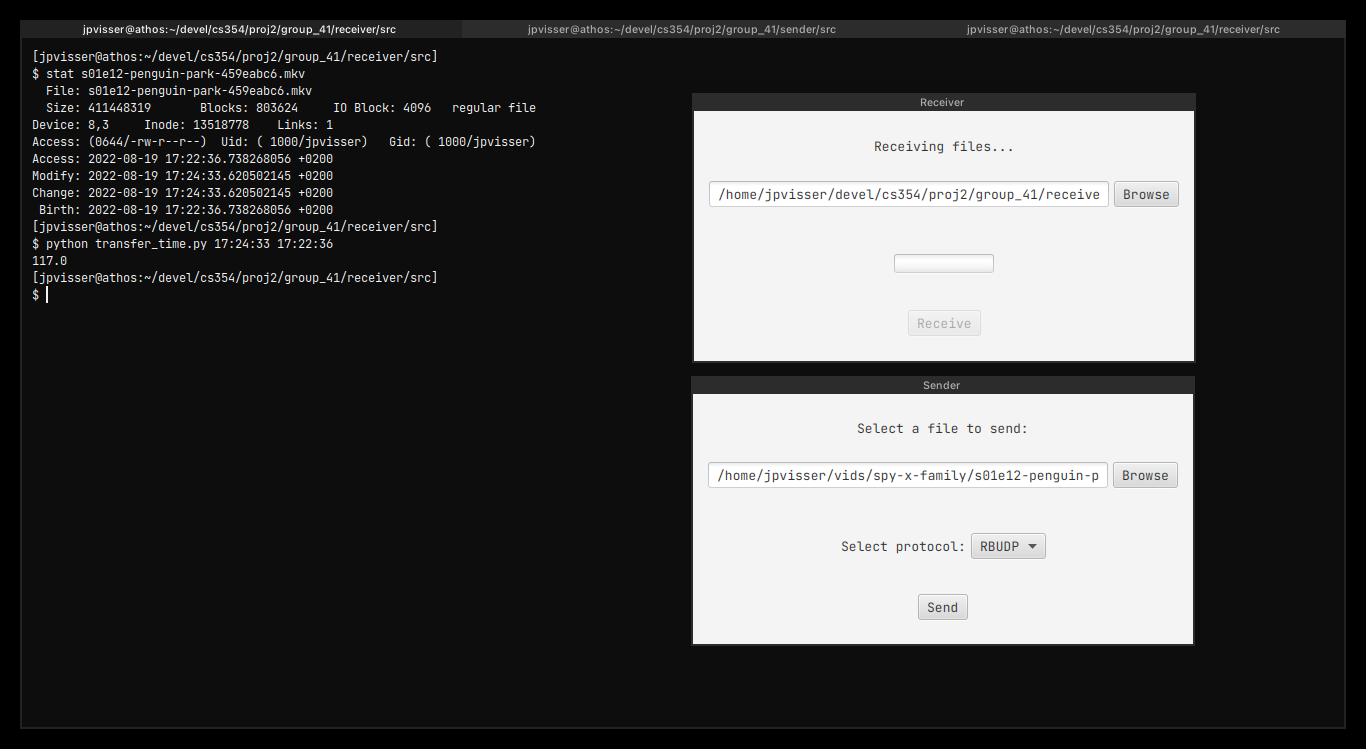
\includegraphics[width=12cm]{exp3-2}
  \caption{The result of running the sender using a packet size of 10000.}
  \label{fig:exp3-1}
\end{figure}

\begin{figure}
  \centering
  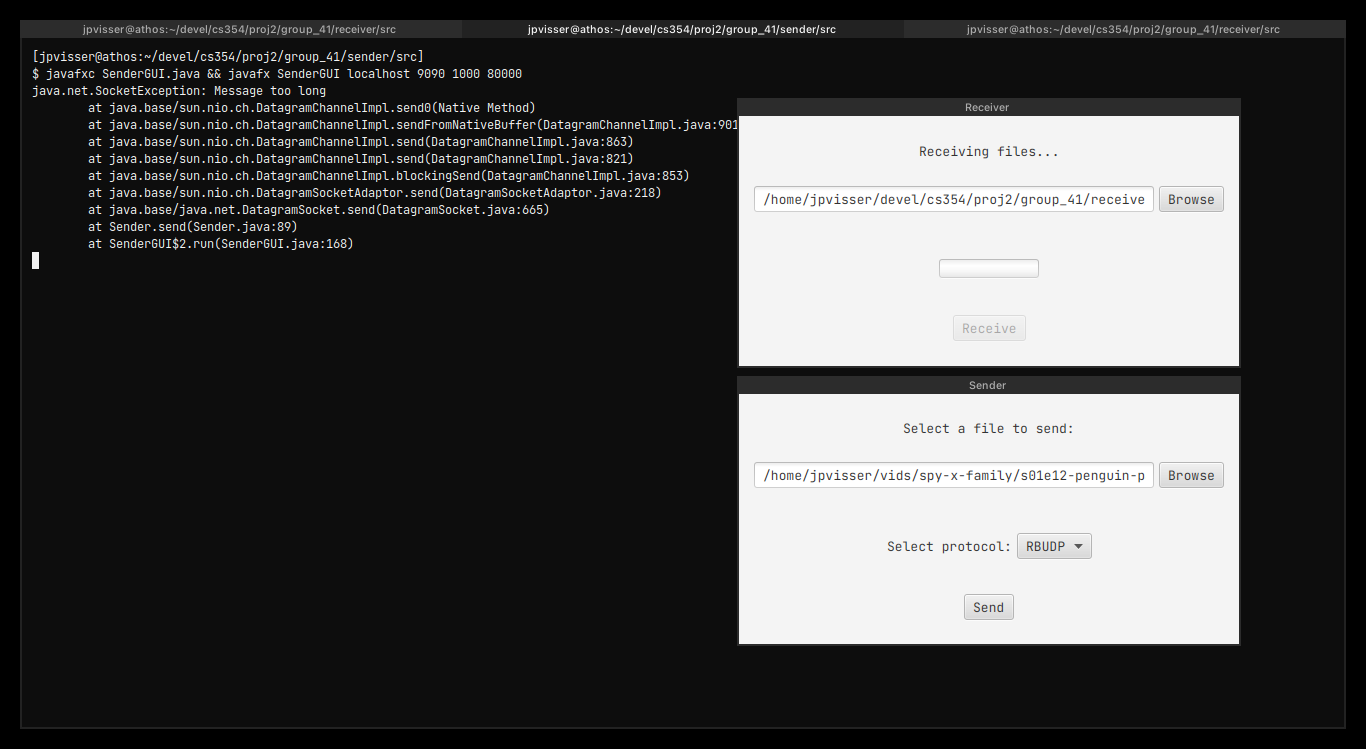
\includegraphics[width=12cm]{exp3-3}
  \caption{\texttt{SocketException} thrown when using a packet size of 80000.}
  \label{fig:exp3-2}
\end{figure}

\subsubsection{Findings}
\label{subsubsec:findings-3}

Our tests partially confirm our hypothesis. In Table \ref{tab:packet-time} it
can clearly be seen that as the packet size doubles, the transfer time gets cut
in half, almost exactly. This indicates a positive correlation between packet
size and transfer rate.

We were, however, not able to test whether there exists a
tipping point where the quantities become negatively correlated: When we
attempted to test the sender with a packet size of 80000, a
\texttt{SocketException} was thrown by the sender (see Figure \ref{fig:exp3-2}).

\begin{table}
  \centering
  \begin{tabular}{@{}rr@{}}
    \toprule
    Packet Size & Time (s) \\
    \midrule
    10000 & 117 \\
    20000 & 61 \\
    40000 & 32 \\
    80000 & NA \\
    \bottomrule
  \end{tabular}
  \caption{The different packet sizes and their associated transfer times in
  seconds when transferring a 393 MB file. The transfer time for packet size
  80000 is indicated as NA, because using a packet size this large caused a
  \texttt{SocketException} to be thrown.}
  \label{tab:packet-time}

\end{table}

% --- Issues Encountered ----------------------------------------------------- %

\section{Issues Encountered}
\label{sec:issues}

\subsection{RBUDP Sender-Receiver Synchronization}
\label{subsec:send-recv-sync}

Designing the algorithms used by the sender and receiver to transfer data via
the RBUDP protocol was difficult, because our aim was to make our implementation
efficient, but also elegant and easy to understand. In the end, we believe the
extra time spent on designing our algorithms paid off, as we ended up with a
succinct implementation that incurs very little overhead.\footnote{This is not
to say our implementation has no shortcomings. In fact, we are aware of several
ways in which it can be refined, but due to time constraints we opted to keep
it as it currently is.}

The bugs we had to deal with in this area were also particularly insidious.

\subsection{Number of Bytes to Write When Using RBUDP}
\label{subsec:num-bytes-to-write}

When transferring data via RBUDP, extracting and writing the bytes received to
disk is mostly an easy task. But once the last part of the file is reached, and
there is not enough data left to completely fill the last packet, it gives rise
to the following problem: How should the receiver be informed of how many bytes
in the last packet actually contains file data that needs to be written?

We discuss how we handled this problem in \S\S\ref{subsec:last-packet}, but we
also thought it worth mentioning here, since it was a difficult design decision
to make. This is also one of the areas where we believe our implementation can
be improved.

\subsection{Connecting and Transferring over the Hamachi VPN}
\label{subsec:connect-transfer-hamachi}

We had considerable difficulty with connecting and transferring files over the
Hamachi VPN, even though our programs performed well when we tested them
locally.

% --- Design ----------------------------------------------------------------- %

\section{Design}
\label{sec:design}

\subsection{The Last RBUDP Packet}
\label{subsec:last-packet}

A simple approach to transferring data via RBUDP is to:\footnote{The approach
presented here is simplified so that we may focus on the problem of
extracting and writing the data from a byte array.}
\begin{enumerate}
  \item Select a set number of packets (blast size) and a set packet size.
  \item Send these quantities to the receiver.
  \item Incrementally read a number of bytes equal to the packet size from the
    file into a byte array. This will constitute a packet.
  \item Once the number of packets created is equal to the blast size, send all
    of the packets to the receiver.
  \item The receiver gets each packet and extracts and writes the same set
    number (communicated to it in step 2) of bytes to the new file.
\end{enumerate}
This works well enough until reaching the end of the file. As explained in
\S\S\ref{subsec:num-bytes-to-write}, when reaching the end of the file, there is
no longer enough bytes left to create a packet with the same size as all of the
other packets that were sent before it. We will also not have the same number of
packets to ``blast".

If this problem goes unaddressed (and we assume the sender
will still send the same number of packets, containing the same number of bytes)
the receiver will end up almost always writing null bytes or junk data to the
end of the file (because the receiver always extracts a set number of bytes
from a set number of packets).

There are a number of ways to address this problem, but we chose to (in addition
to sequence numbers) include the number of data bytes at the start of the packet
(after the sequence number). This way the receiver will always know exactly how
many bytes of those it receives in a packet to write to disk.

Our solution obviously has some (maybe even significant) overhead associated
with it, but we settled on it due to the simplicity of the code required to
implement it, as well as time constraints.

% --- Compilation and Execution ---------------------------------------------- %

\section{Compilation and Execution}
\label{sec:comp-exec}

It is assumed that the project will be run on Linux from a Bash shell.

\subsection{Dependencies}
\label{subsec:deps}

In order to compile and run the sender and receiver the following dependencies
must be installed and available on the \texttt{PATH}:
\begin{itemize}
  \item OpenJDK 18.0.2
  \item OpenJFX 18.0.2.u2-1
  \item Gradle 7.5
\end{itemize}

\subsection{Receiver}
\label{subsec:deps-receiver}

The receiver can be compiled and executed by following the next steps:
From the project root directory \texttt{cd} into the \texttt{receiver} directory.
Execute the script \texttt{run.sh}.

\subsection{Sender}
\label{subsec:deps-sender}

From another terminal window, follow the same steps for the receiver, but in
step 1 \texttt{cd} into the \texttt{sender} directory, and, when executing
\texttt{run.sh}, supply as argument the IP address or hostname of the machine or
network the receiver is running on.

% --- Libraries -------------------------------------------------------------- %

\section{Libraries}
\label{sec:libs}

We used only the following libraries for this project:
\begin{itemize}
  \item Java Standard API
  \item JavaFX
\end{itemize}

\end{document}
